\documentclass[a4paper,11pt]{article}
\usepackage[english, french]{babel}
\usepackage[T1]{fontenc}
\usepackage[utf8]{inputenc}
\usepackage{hyperref}
\usepackage{graphicx}
\usepackage{eurosym}
\usepackage{subcaption}
\usepackage{framed}
\usepackage{sectsty} %pour les commandes en début de section

\sectionfont{\clearpage}
\counterwithout{figure}{section}
\counterwithout{table}{section}

\begin{document}

%%%%%%%%%%%%%%%%
\section{Introduction}

\subsection{Aim of this paper}

In the field of digital humanities, the great concern is to build an accurate, reliable and useful digital representation of analogical material. For that reason, methodological papers focus on the main steps of that process: digitalization, layout detection, character recognition, spelling correction, names recognition, text encoding, design of ontologies. Natural Language Processing and Automatic Classification can be of some use, for instance when it comes to detecting errors -- actually, NLP techniques are built-in parts of modern OCR algorithms. However, they are mostly seen as tools, and thus their efficiency is assessed in a pretty straightforward way: how accurate is the result they provide with regard to the initial material.

When it comes to research in Data Science though, things can get quite tricky. There is hardly a unified framework to answer questions such as: is topic modeling giving me good insights about the evolution of the concerns my corpus deals with over time? What is a relevant division of my corpus according to time periods, geographical zones, political lines? More generally, it might be quite difficult to be sure that the insights we get from exploratory analysis are not misleading, especially when we are dealing with amounts of data that make direct verifications virtually impossible.

In this paper, we aim to address several kinds of problems that historians have to consider  when dealing with large amounts of digital data:
\begin{itemize}
	\item how can we select relevant data throuh huge amounts of materials?
	\item what kind of visualization might give the best insights about the dispersion of the data?
	\item how is it possible to come with meaningful variables and to classify the data to a high degree of certainty?
	\item what is a relevant method to display evolutions throughout time?
\end{itemize}

\subsection{Previous works and perspectives}

\subsection{Outline}

This article is divided into four sections, each one about one category of methods. In the first section, we deal with supervised classification, and how to use it identify relevant information in a huge corpus. In the second section, we start tackling the high dimension through the angle of visualization: how to represent information in a way which is meaningful and as little misleading as it is possible -- both for exploration and explanation purposes. In the third section, we investigate some methods which are specific to NLP and help building accurate variables beyond the simple frequencies. Finally, the fourth section is devoted to the analysis of the time component in different kind of corpora. 


\subsection{Data}

Although this paper is mostly a methodology paper, we will focus on one single source, namely the parliamentary reports form french Third Republic, with the hope of showing some insights about the corpus that researches in political history might find interesting per se. From 1881 to 1940 and the fall of the Republic, the debates in the lower chamber of french Parliament have been recorded and published in the \textit{Journal Officiel}. In the early 2010s, the archivists from the french national library (BNF) have digitalized these texts, stored them in a freely accessible database on \textit{Gallica}[REF], together with some precious metadata, and finally performed automatic transcription (OCR) on them. They have made available online these texts in XML format[REF]; hereafter we will refer to this corpus as OCR-12. However, these transcriptions were not manually proofread, and, due to the early technology that was used back then, were not absolutely accurate (see figure~\ref{fig:data}). Thanks to grants from BNF-Datalab and INRIA, a team of researchers (INRIA-Almanach, LARHA and Epitech MNSHS) have been able to come up with a new version of the transcription with greater accuracy, though only for the period 1890-1900. Most of the examples in this article are taken from that recent transcription, which we call OCR-21, while for some long-term analysis we will have to use OCR-12.

\begin{figure}
\hyphenpenalty=1000
\begin{subfigure}{\textwidth}
\begin{center}
	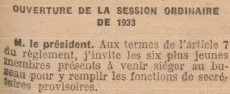
\includegraphics[width=11cm, height=11cm, keepaspectratio]{./img/jo33}\\
	\caption{Original (digitalized) text}
\end{center}
\end{subfigure}
\begin{subfigure}{0.45\textwidth}
	\begin{framed}
OUVERTURE DE LA SESSION ORDINAIRE DE 1933 M. le président. Aux termes de l'article 7 5U règlement, j'invite les six plus jeunes SQfâinbres présents à venir siéger au buu pour y remplir les fonctions do secrér "V.l!lles provisoires.
\end{framed}
	\caption{OCR-12 version}
\end{subfigure}
\begin{subfigure}{0.1\textwidth}
	\hspace{0.8cm}
\end{subfigure}
\begin{subfigure}{0.45\textwidth}
	\begin{framed}
OUVERTURE DE LA SESSION ORDINAIRE DE 1933\\
M. le président. Aux termes de l'article 7 du règlement, j'invite les six plus jeunes membres présents à venir siéger au bureau pour y remplir les fonctions de secrétaires provisoires.
	\end{framed}
	\caption{OCR-21 version}
\end{subfigure}
\caption{Issue from the parliamentary report, January 1933}
\label{fig:data}
\end{figure}


\section{Building the Data}

In this section we will address the question of identifying texts that a relevant for a given purpose

\subsection*{Supervised classification}

Let us assume we dispose of a huge corpus, and we want to find out all the documents that deal with a certain issue, for instance the role of the Church within the State. We cannot extensively go through all documents and decide one after the other. In addition, we cannot just identify a few keywords, for deciding in advance which ones are necessary would probably lead to a lot of mistakes and misses. One solution is to train an algorithm on a sample and then apply it to the rest of the corpus.

Formally, we consider a problem of supervised classification. We have two classes, say 0,1 : 1 stands for the documents that are relevant to our purpose while 0 stands for those who are not. We divide at random the data set into three parts, (let us say for the sake of example, that they stand for respectively 6\%, 4\% and 90\% of the corpus) that we call the training set, the validation test and the test set. The analysis now consists of the following steps:
\begin{enumerate}
	\item Manually label all the texts in the training and validation sets, so that we know for sure which ones are relevant to the topic and which ones are not.
	\item Train various algorithms and parameters on the train set and monitor their performance on the validation test.
	\item Once the performance indicators are accurate enough, use the trained algorithm to find out which texts in the test set belong to the expected class.
\end{enumerate}

\begin{figure}
	\begin{subfigure}{\textwidth}
		\begin{tabular}{|p{11cm}|l|}
		\hline
		X & Y\\
		\hline
		A ceux qui ne veulent pas abroger le Concordat et la loi de l'an X, je dis : Sur ce point, vous devez être avec nous; il doit y avoir unanimité dans cette Chambre parmi les républicains pour séculariser les biens des congrégations religieuses. (...) & 1\\
		\hline
		En effet, un traité a été conclu avec la république Sud-Africaine, celui qu'invoquait au début de la séance M. le ministre des affaires étrangères comme nous liant, par suite de la clause de la nation la plus favorisée, avec les autres pays européens. (...) & 0\\
		\hline
		\end{tabular}
		\caption{Excerpt from the labeled table}
	\end{subfigure}

	\begin{subfigure}{\textwidth}
	\begin{center}
		\begin{tabular}{|l|l||l|l||l|l|}
		\hline
		word & score & word & score & word & score\\
		\hline
		mot1 & 17.5 & mot3 & -8.6&  mot5 & -3.9 \\
		mot2 & 12.3 & mot4 & 7.6 & mot6 & 3.3\\
		\hline
		\end{tabular}
	\end{center}
	\caption{Main keywords automatically identified by the Naive Bayes algorithm [TODO ; placeholder pour le moment]. A positive score is in favor of Y=1 while a negative one is in favor of Y=0}
	\end{subfigure}
\caption{Some insights about texts dealing with the role of the Church within the State}
\label{fig:naifbayes}
\end{figure}

\subsection*{Assessing the quality of a classification}

The ability of an algorithm to correctly predict which text belongs to a given class among the large test set -- which we cannot directly assess, for it is too big -- can be inferred from its ability to predict on the validation set. Note that this induction only works if the sets are parted randomly: otherwise, the indicators might be biased. This being said, let us consider the indicators we dispose of for that assessment.

First and most straightforward indicator is called accuracy: how many times does the algorithm succeed at predicting the accurate value of the class. A score of 50\% means the algorithm is not better than pure randomness and thus can be discarded, while a 100\% is a perfect prediction. However an accuracy at 90\% means nothing per se. Indeed, consider the class of all the texts dealing with Church problems among the parliamentary reports. These texts represent only 182 among 7473, that means 2.44\%. Thus it is possible to achieve 97.56\% accuracy by predicting that no text at all is about the Church. Thus we will rather rely on two slightly more sophisticated measures: the Confusion Matrix and the Receiver Operating Characteristic (see Figure~\ref{fig:cm_roc}). The confusion matrix simply plots the predicted classes against the real ones, allowing one to simultaneously check the ability of the algorithm to assess all classes. On the other hand, the ROC curve plots the true positive rate against the false positive rate as the algorithm builds predictions by decreasing order of certainty. It can be used both for ranking algorithms (the further a curve is from the diagonal line the better) and for deciding until which portion of the sample the algorithm can be trusted (at some point the ratio of true positive vs false positive becomes too close to a randomness)

\begin{figure}
	\begin{subfigure}{0.5\textwidth}
		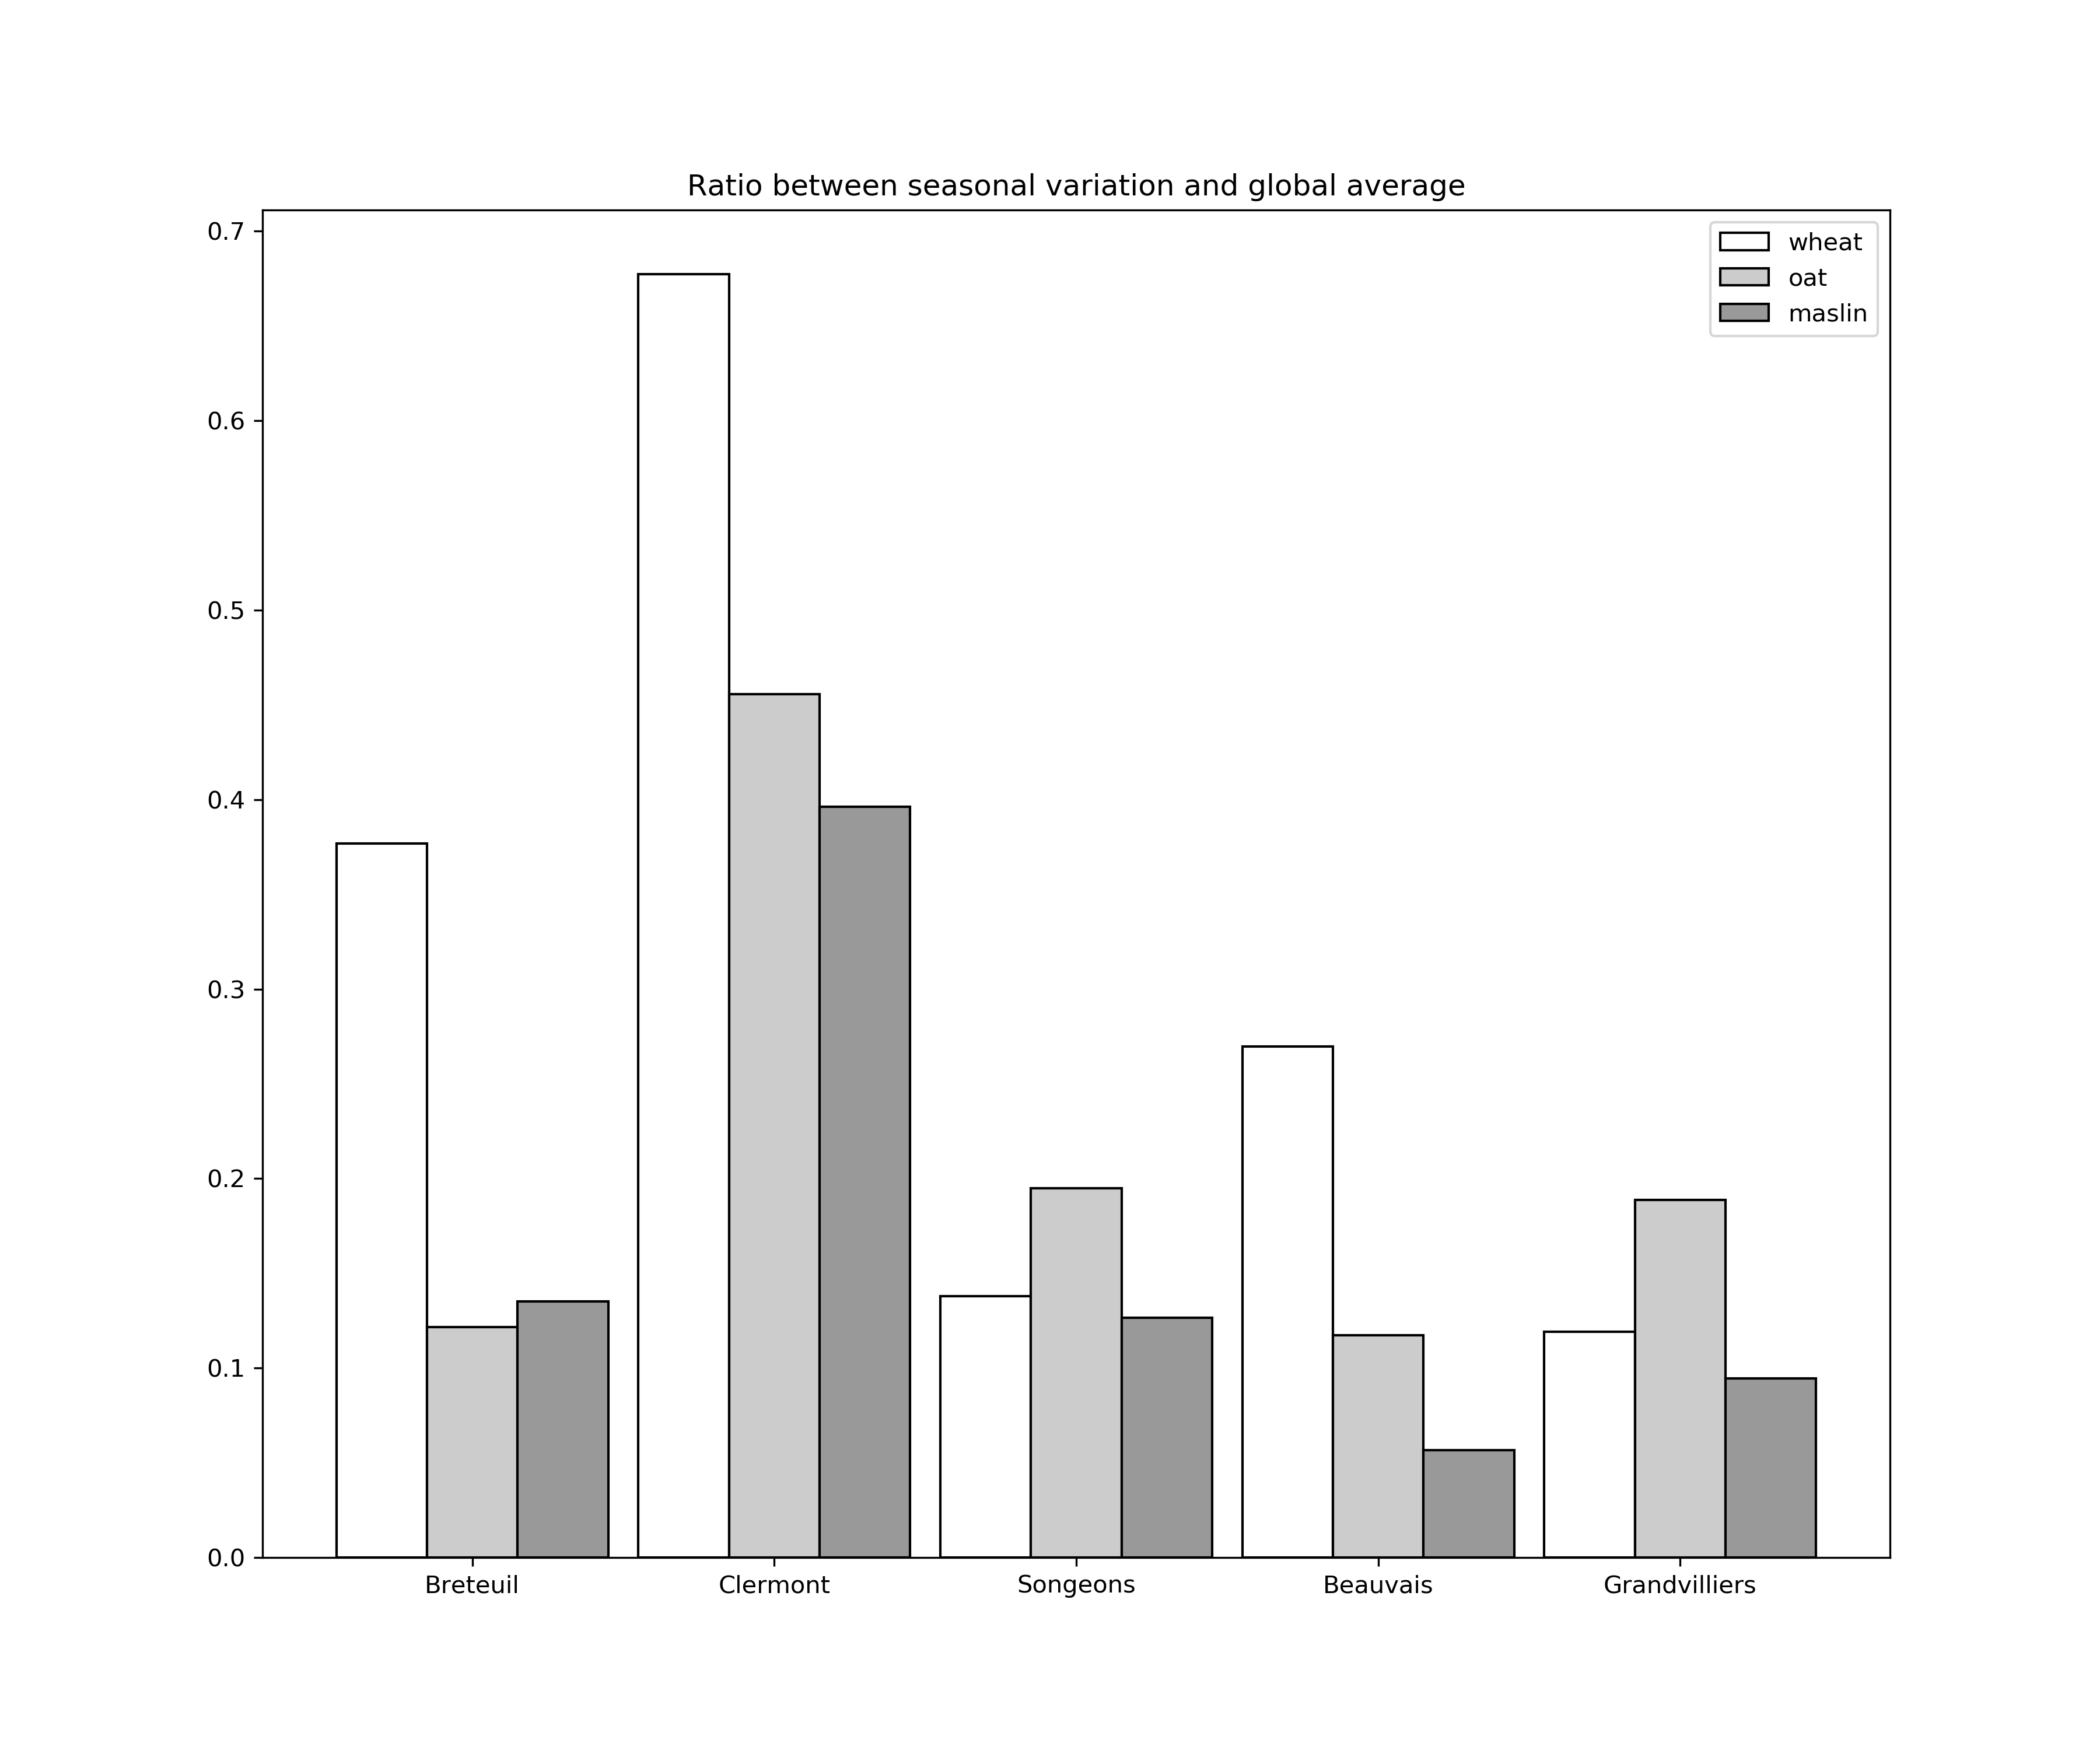
\includegraphics[width=5.5cm, height=5.5cm, keepaspectratio]{./img/placeholder}
		\caption{Confusion Matrix [placeholder]}
	\end{subfigure}
	\begin{subfigure}{0.5\textwidth}
		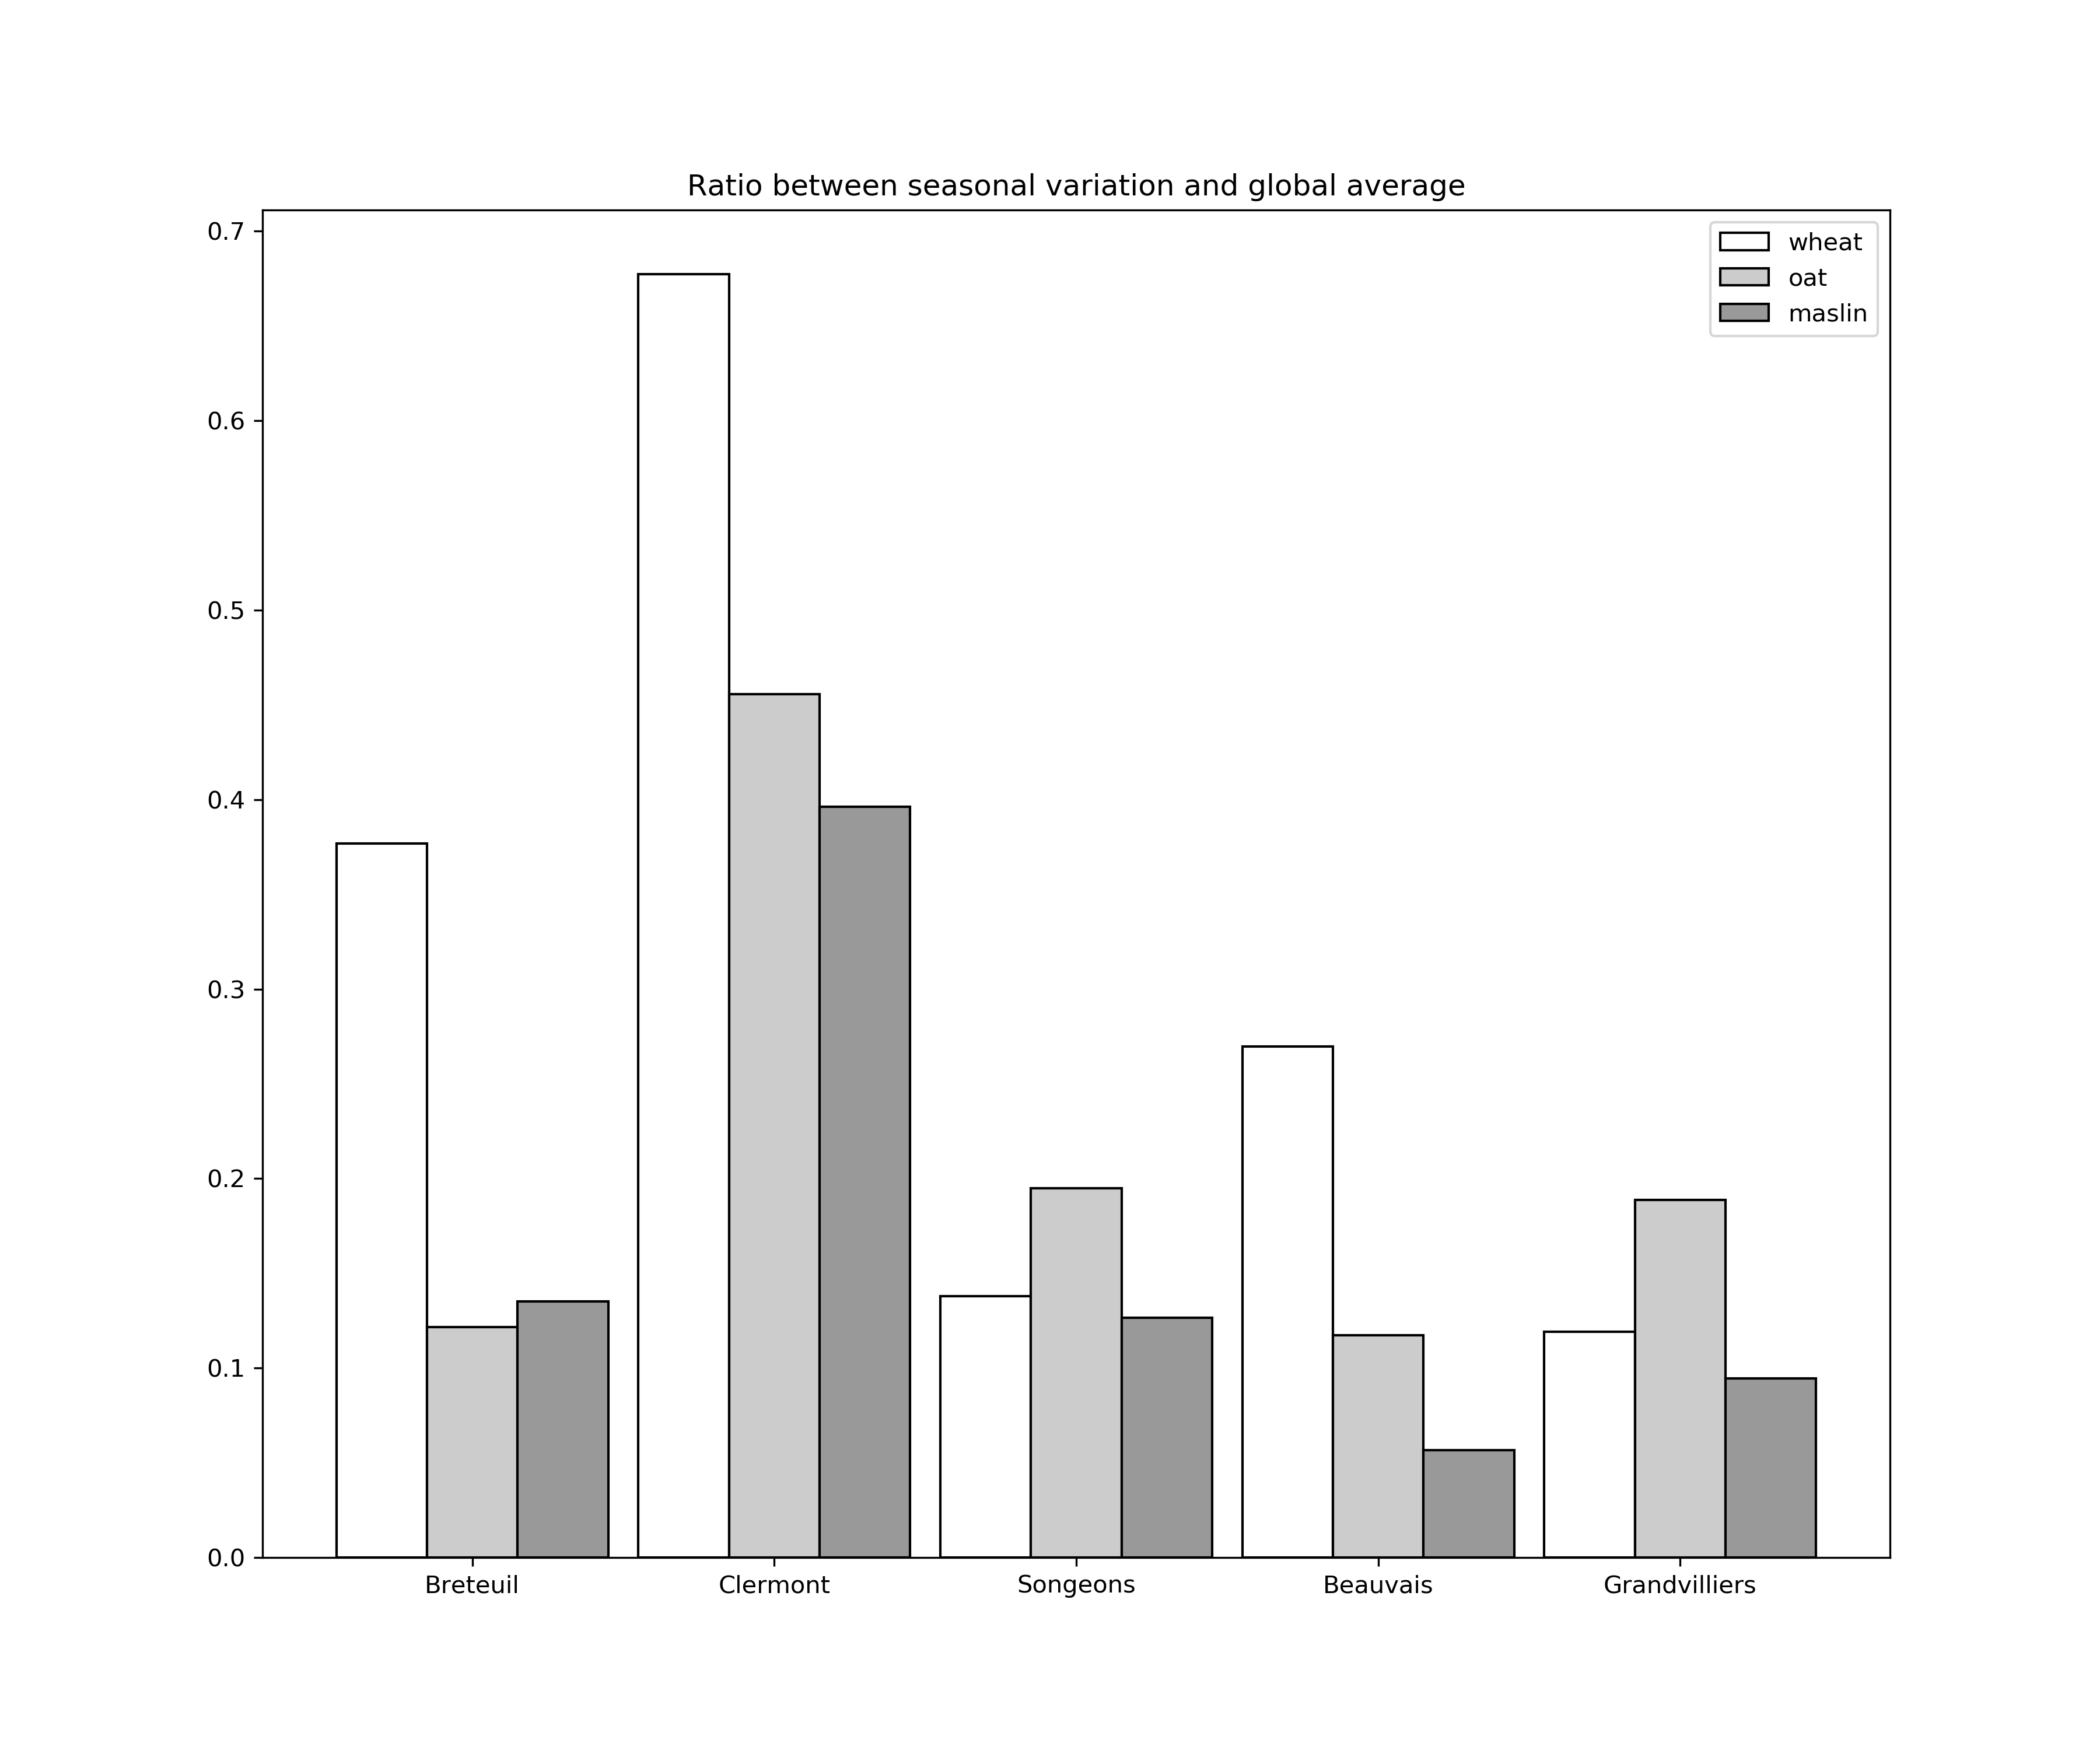
\includegraphics[width=5.5cm, height=5.5cm, keepaspectratio]{./img/placeholder}
		\caption{ROC [placeholder]}
	\end{subfigure}
\caption{Some indicators about the respective quality of a Naive Bayes (red) and a SVM (blue) algorithm for predicting Church-related texts, assessed on the validation test.}
\label{fig:cm_roc}
\end{figure}

\begin{figure}
	\begin{subfigure}{0.5\textwidth}
		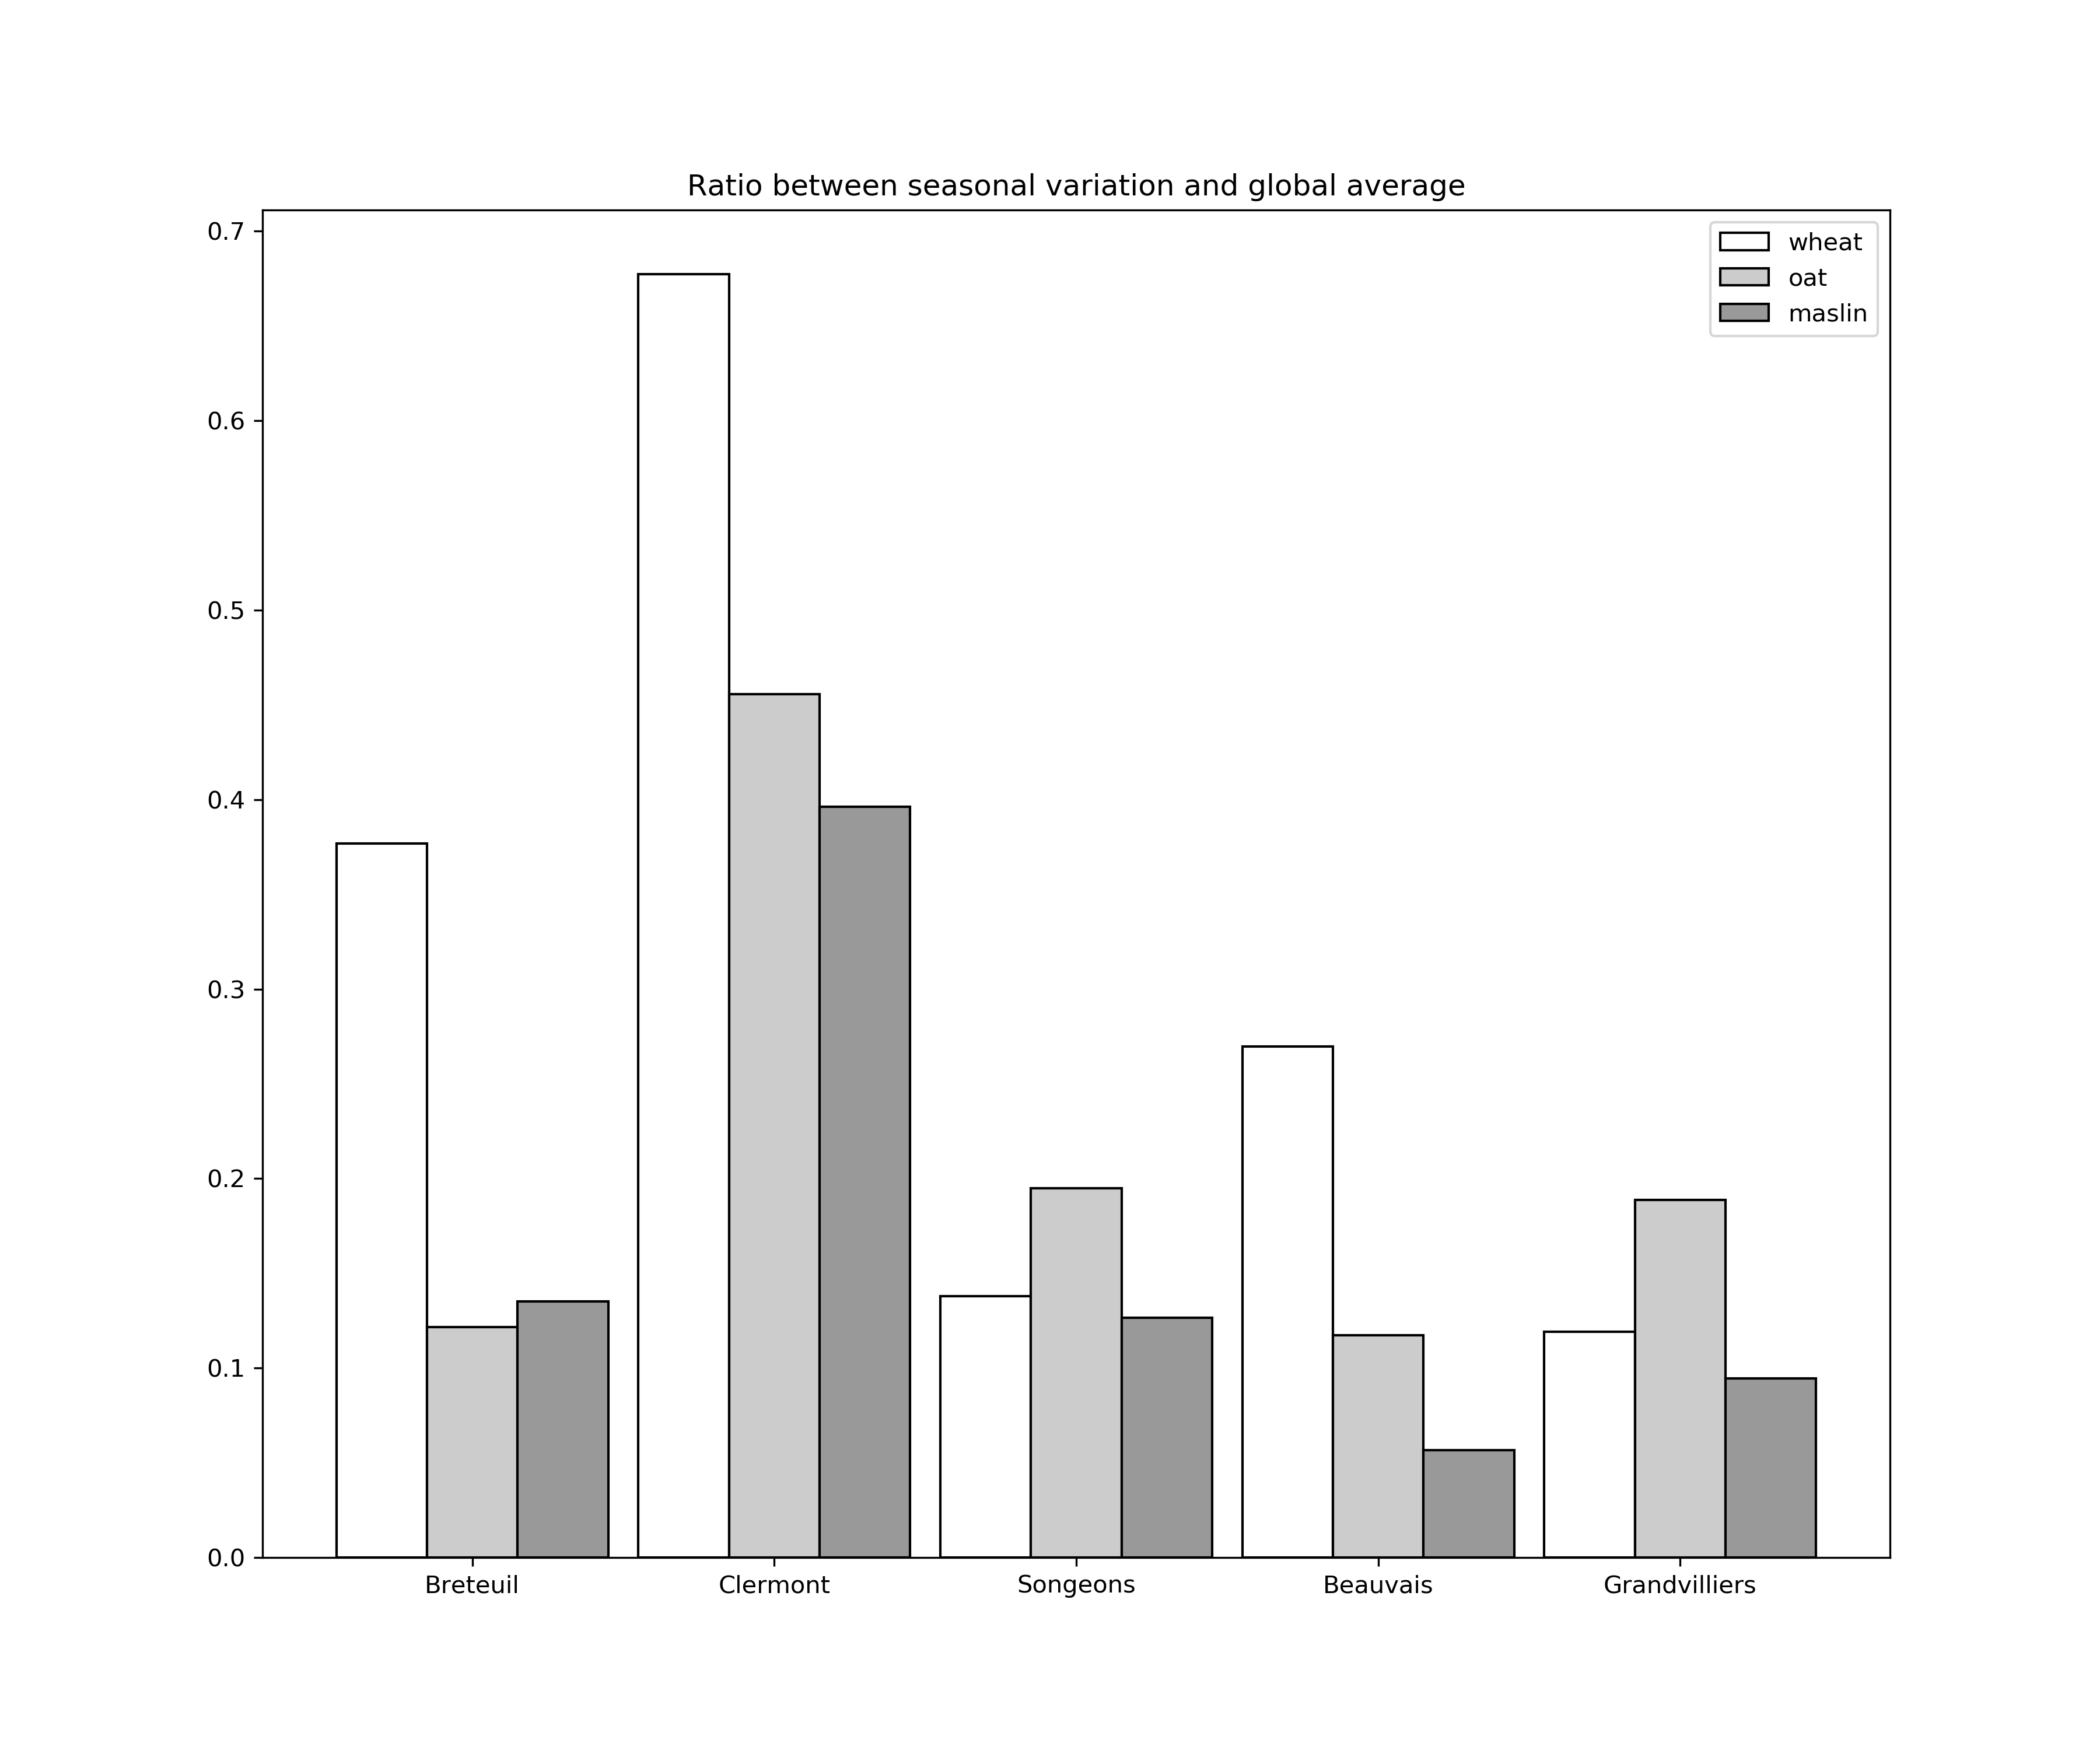
\includegraphics[width=5.5cm, height=5.5cm, keepaspectratio]{./img/placeholder}
		\caption{Naive Bayes classification [placeholder]}
	\end{subfigure}
	\begin{subfigure}{0.5\textwidth}
		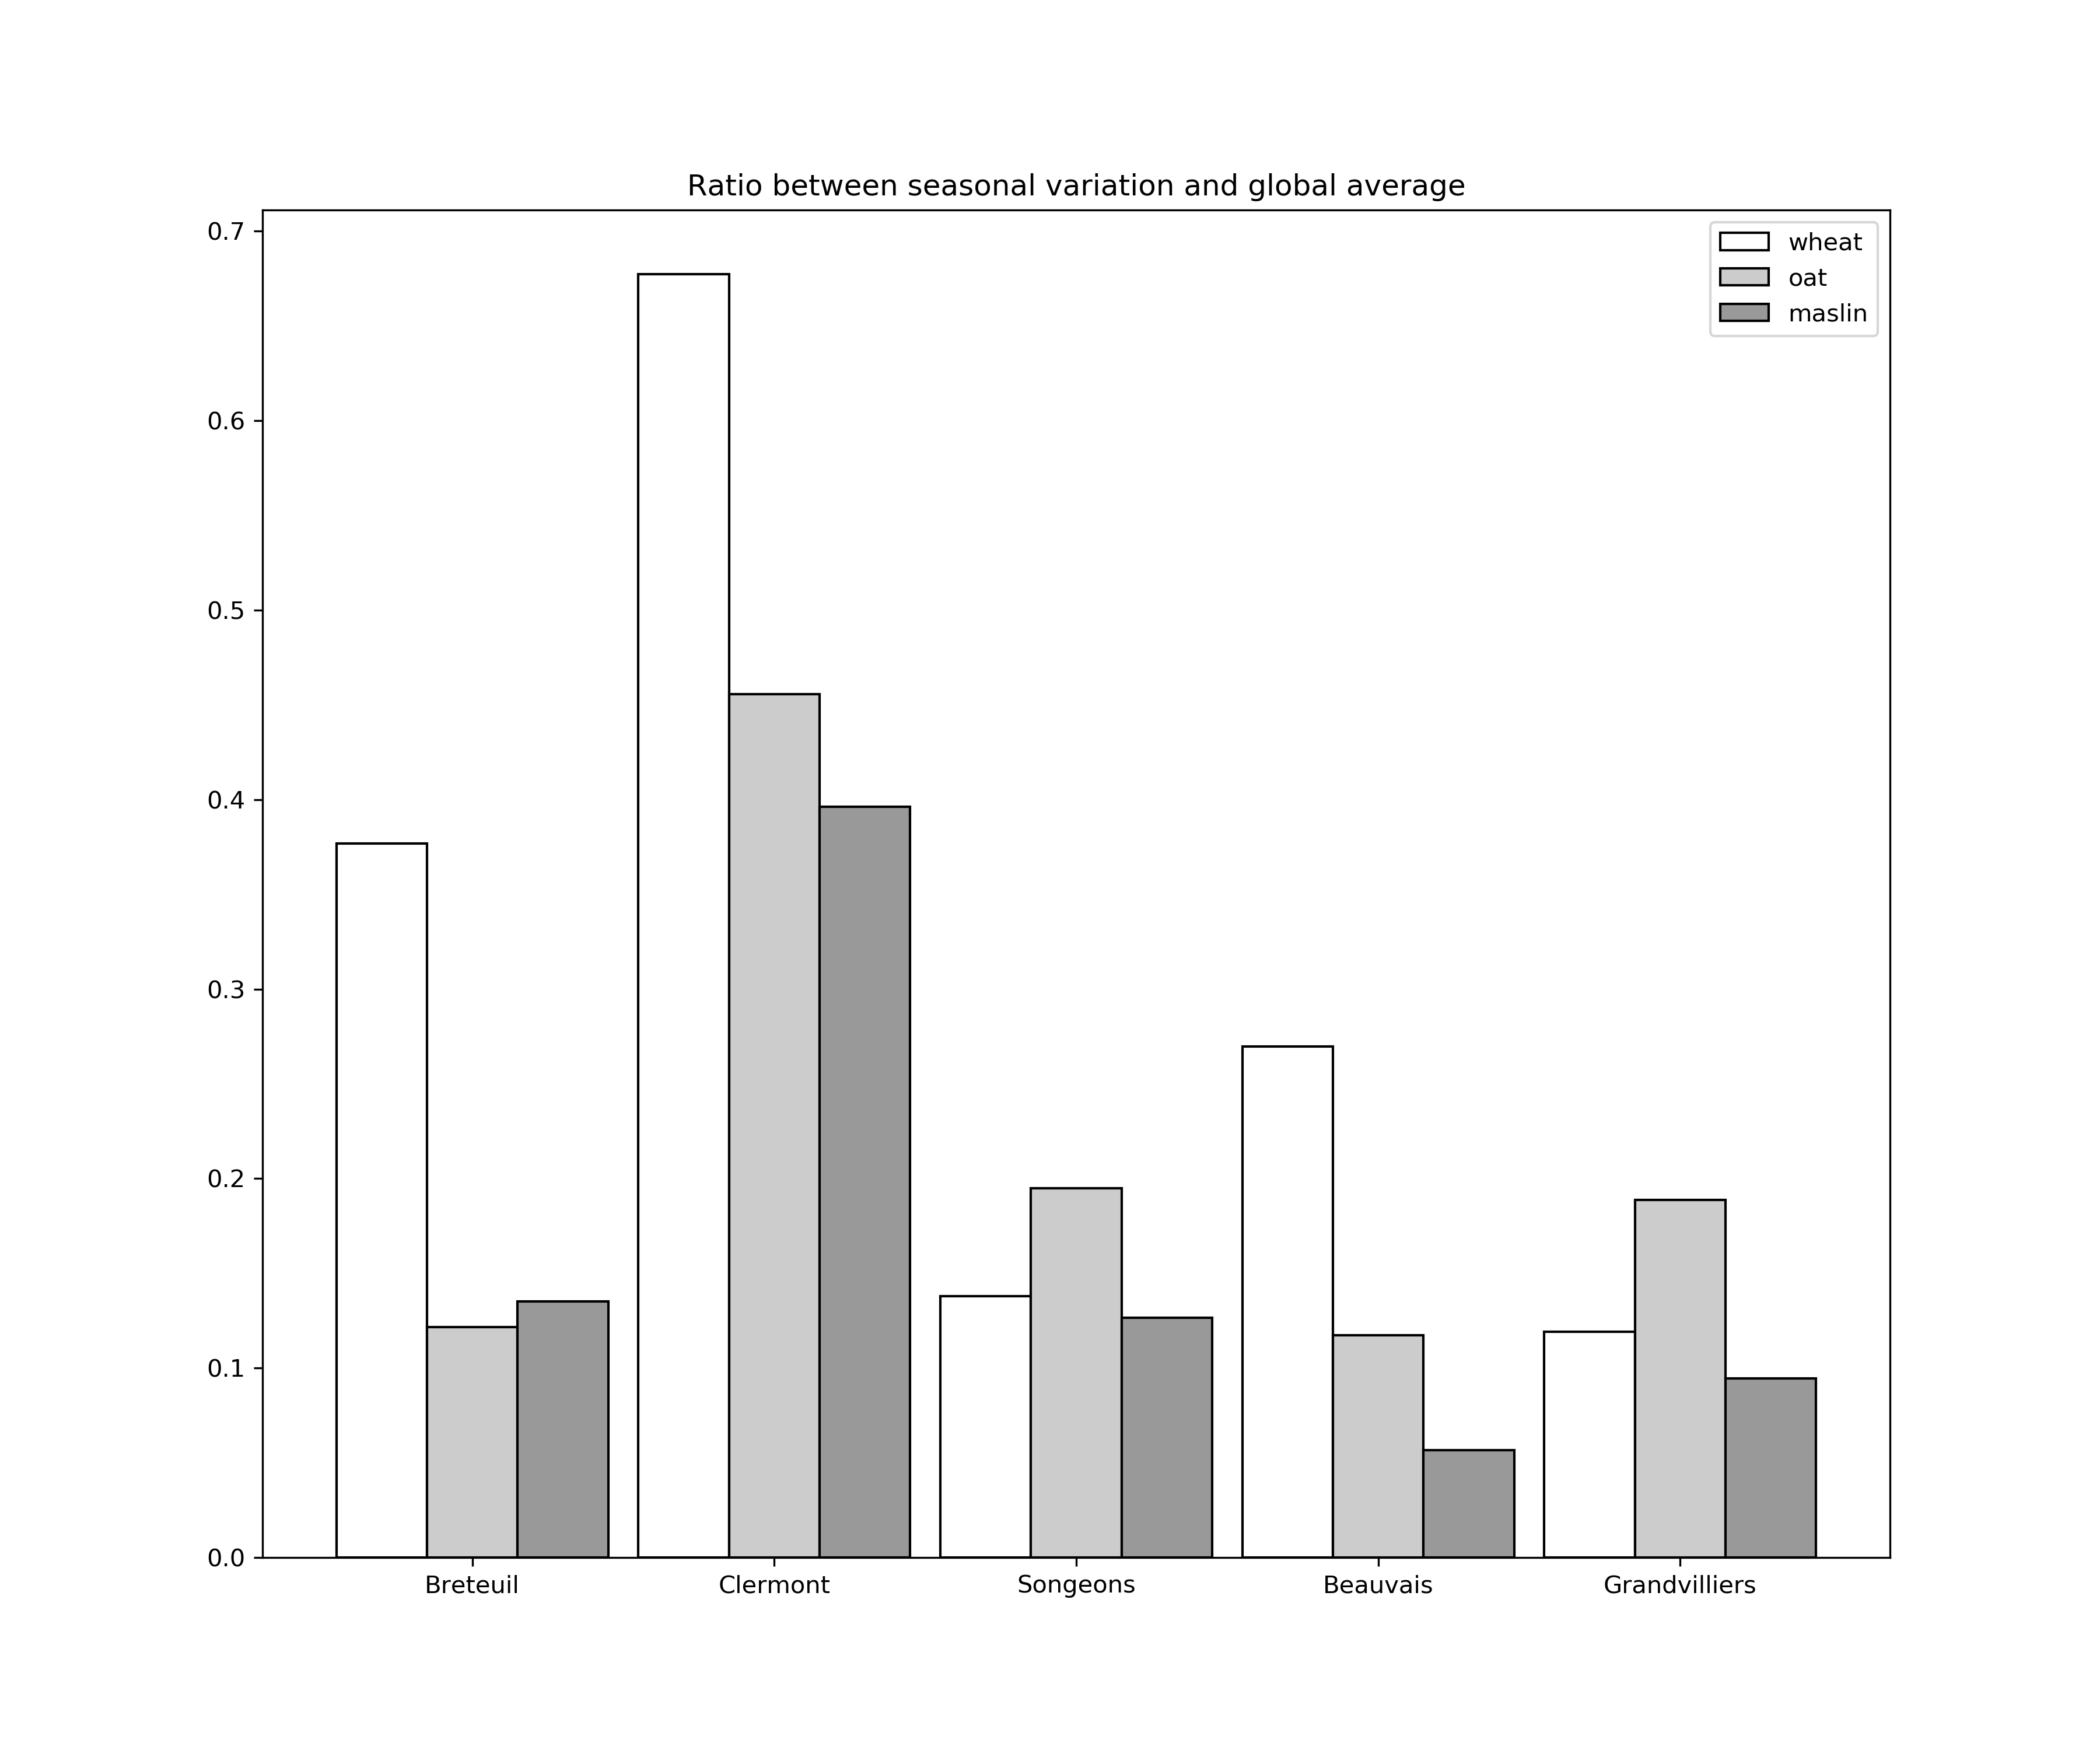
\includegraphics[width=5.5cm, height=5.5cm, keepaspectratio]{./img/placeholder}
		\caption{Support Vector Machine [placeholder]}
	\end{subfigure}
\caption{The two axes are the most prominent features and the colors stand for the two classes (green=1, orange=0). Dots with a thick black border are those from the training set, while others have been predicted.}
\label{fig:svm_bn}
\end{figure}


\section{The dimension problem, part 1:  Visualization}

In many social sciences, we are used to dealing with tabular data. Any data unit can be seen as a vector in some multi-dimensional space. For instance, our corpus can be described as a table of pages, with some meta-data information, and for every word of the vocabulary the number of occurences within the page (Table~\ref{exdata}). When it comes to this kind of representation, the dimension of the space can be huge, tens of thousands of columns. Hence it is difficult to provide a 2-D visualisation of that data, for instance for the purpose of understanding which pages have similar content, deal with the same topics, or might have been written in close context. 

\subsection*{Limits of PCA}

Among the most popular tools is the Principal Component Analysis (PCA). Basically the PCA performs a rotation inside the data space, in such a ways that $i$-th axis has maximal variance among the subspace where axis $1$ to $i-1$ have been removed. This might come in handy when the first axes are able to capture a significant part of the overall variance, as it is often the case with small-dimension or highly-correlated data. However, when it comes to textometry, such conditions are not met so frequently, and thus the tool can be misleading.

Figure~\ref{fig:acp_pb} is an example of such a confusion. Here we are displaying the results of a PCA trained on the documents issued in 1882 -- their names are encoded in the format MONTH-DAY (+\_num in case of several documents in a single day), based on the frequency of words in each text. We can ignore the colors for the moment and focus on the proximity of some nodes. Formally, the distance between two documents is equal to the sum of the squares of differences in frequencies over all the vocabulary $D(a,b) = \sum_{w \in \mathcal{V}} (f_w(a)-f_w(b))^2$. Although they look very close in the PCA the documents 02-23 and 02-13 are actually quite distant as we can see from the table. Symmetrically, the documents 02-23 and 05-11 are shown at long distance from each other in the PCA while they are actually closer neighbors than the previous pair.

These false impressions could be corrected by looking at the other axes from the PCA -- here the third one mostly, but watching simultaneously several graphs and pondering them with the contribution of every axis does not make the PCA a very practical tool for understanding proximities on a global scale. Therefore, we want to emphasize the importance of two methods that may be good replacements or complements to PCA, namely: non-linear transforms and automatic clustering.

\begin{table}
\begin{tabular}{|l|l|l|l|l|l|l|}
\hline
page & date &  "président" & "terme" &  "article" & "règlement" & $\ldots$ \\
\hline
6829 & 1933-01-10 & 24 & 1 & 5 & 3 & $\ldots$\\
\hline
\end{tabular}
\caption{Excerpt from a line in the database describing one document}
\label{exdata}
\end{table}

\begin{figure}
\begin{subfigure}{0.6\textwidth}
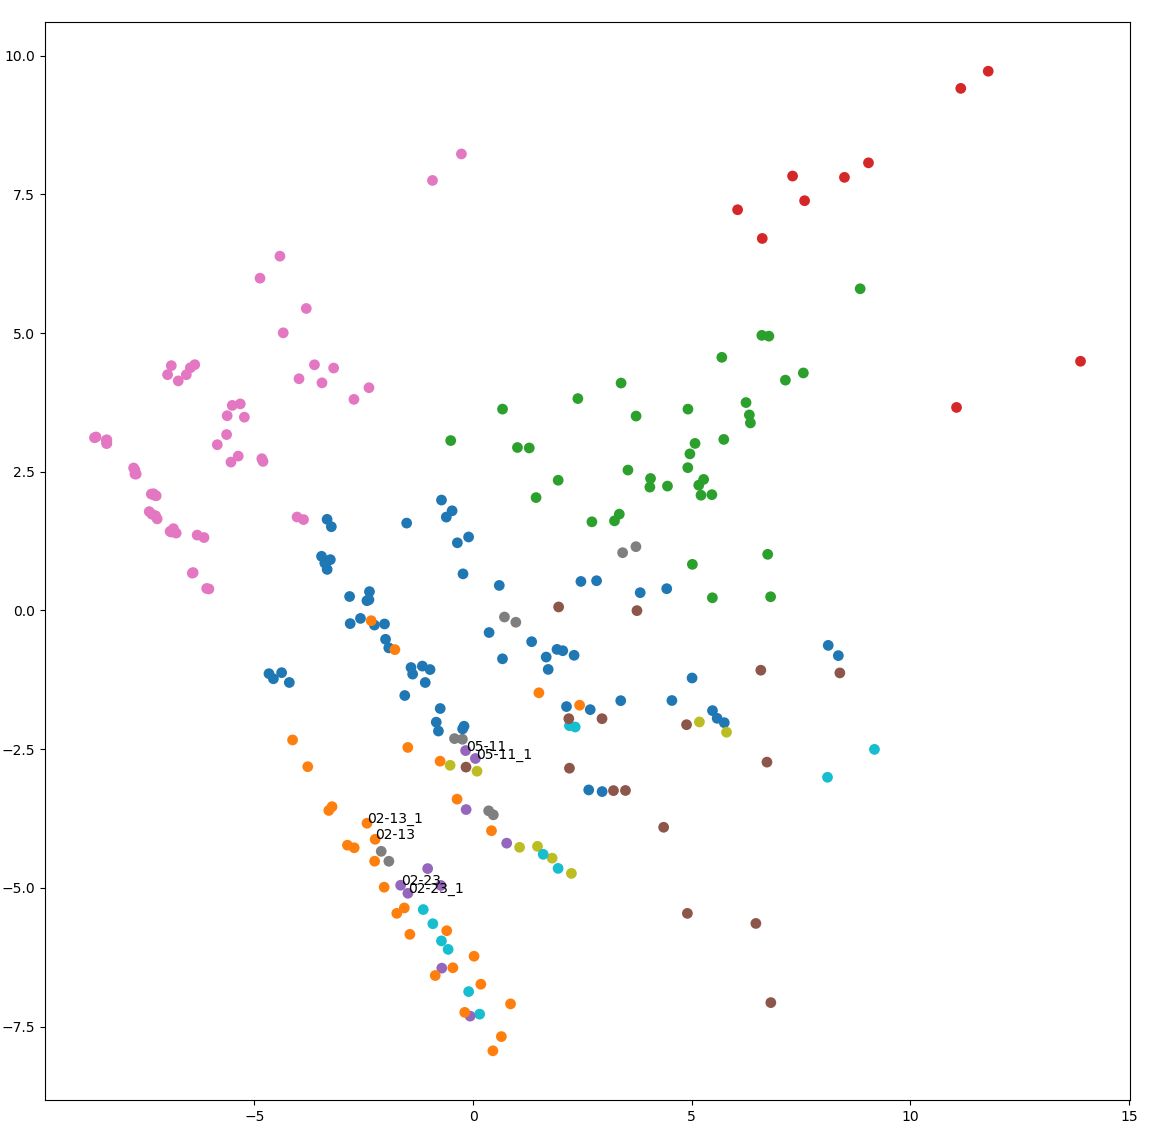
\includegraphics[width=7.5cm, height=7.5cm, keepaspectratio]{./img/acp_1}
\end{subfigure}
\begin{subfigure}{0.4\textwidth}
\begin{tabular}{|l|l|}
\hline
distance & 02-23 \\
\hline
02-23	& 0.\\
02-23\_1	& 0.26\\
05-11	& 1.80\\
05-11\_1	& 1.80\\
$\ldots$	& $\ldots$\\
07-18	& 2.38\\
07-18\_1	& 2.39\\
$\ldots$	& $\ldots$\\
02-13	& 2.98\\
02-13\_1	& 2.99\\
\hline

\end{tabular}
\end{subfigure}
\caption{Contrary to what its seems in the PCA, the documents 02-23 and 02-13 are actually quite distant and 02-23 is much closer to 05-11.}
\label{fig:acp_pb}
\end{figure}

\subsection*{Non-linear methods}

A Self-Organizing Map (SOM) is a non-linear and stochastic projection of the data space on a low-dimension (usually 2-D) grid [REF]. The SOM algorithm is an iterative algorithm, which takes as input a dataset and computes units (the cells of the grid) which define the map. The grid is at first dispatched randomly in the dataspace; then a sequence of steps is computed. At every step, one data is chosen at random and attributed to the closest cell, which is moved in the dataspace in order to have the data in the center of the cell. Neighboring cells are also moved in that direction, though along only a fraction of the distance. One could think to the grid as if it was drawn on a piece of fabric twisted by pushing a finger on some point. We know that self-organization is reached at the end of the algorithm, which implies that close data in the input space have to belong to the same class or to neighboring classes, that is to say that they are projected on the same cells or on neighboring cells on the map (see Figure~\ref{fig:som_pb} for an example).\\

\begin{figure}
\begin{center}
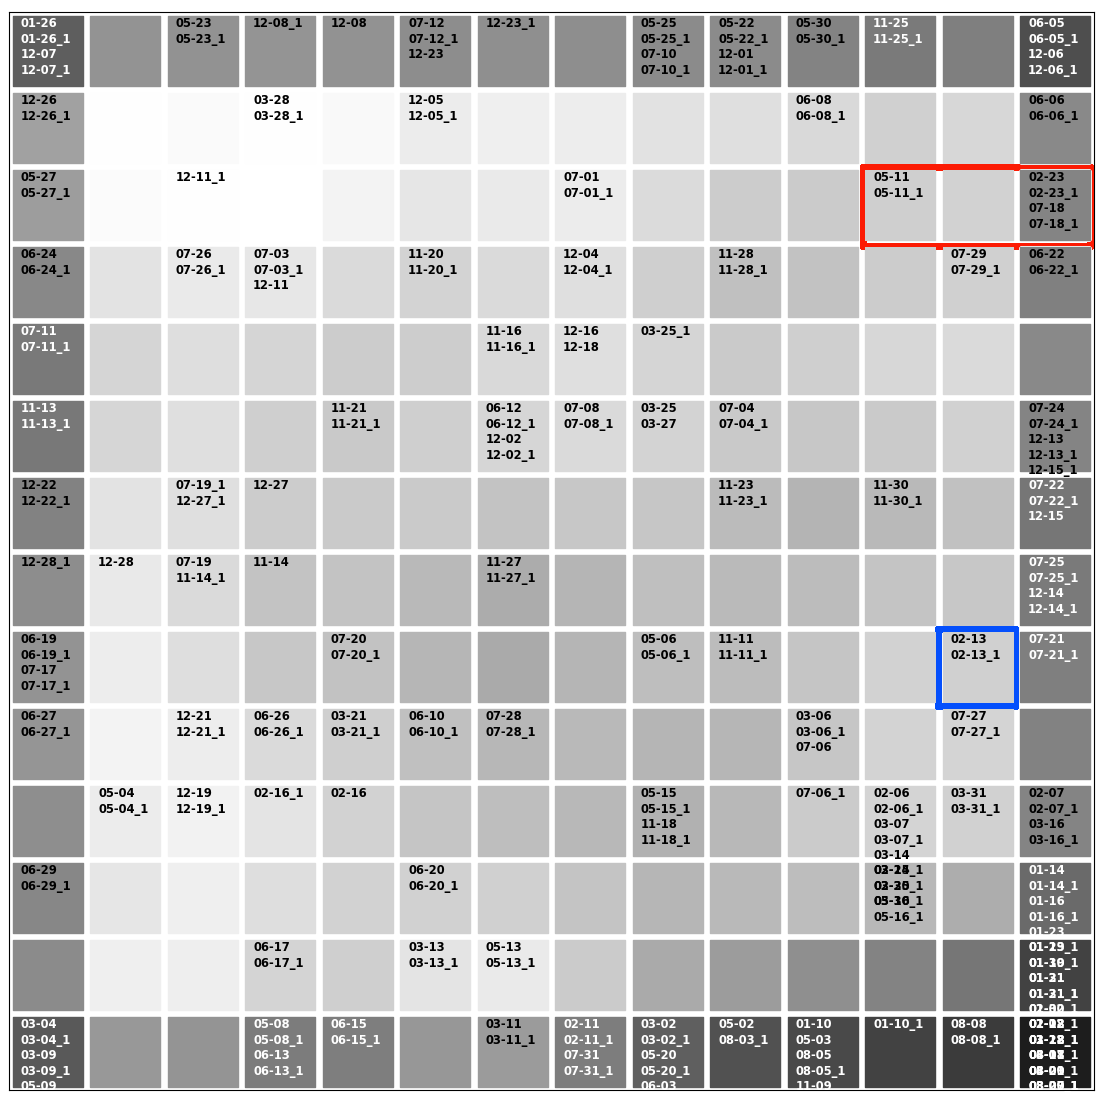
\includegraphics[width=11cm, height=11cm, keepaspectratio]{./img/som_1}
\caption{The documents which are the closest to 12-23 are in neighboring cells}
\label{fig:som_pb}
\end{center}
\end{figure}

Notice that the reciprocal is not true: as any dimension reduction method, a SOM can produce fake similarity.[TODO mentionner alternatives, comme gaz] In order to tackle this problem, we can introduce additional visualisation elements. First one is the distance between cells, as it is displayed on Figure~\ref{fig:som_pb}. The distance between a cell and its neighbors is highlighted by the gray scale : the darker, the further. Another efficient tool is clustering, also called unsupervised classification.

\subsection*{Clustering as a tool for visualization}

The aim of a clustering is to divide a dataset in clusters of vertices that are close to each other, according to some metrics. A clustering can be illustrated by a choice of colors, shapes or markers, each coding for a different class. The borders of these classes are not only providing additional information to the graph, but can also help spotting problems. For instance, the colors in Figure~\ref{fig:acp_pb} represents the different classes from an Agglomerative Clustering with 8 components. The orange, violet and lightblue dots seem very intricated, while they are in reality pretty well divided apart\footnote{Once spotted, this can be verified pretty well along the 3rd axis of the PCA. However, figuring the overall division with the only help of the PCA axes would have been extremely difficult.}. Similar information could be added on the Self-Organizing map in Figure~\ref{fig:som_pb}.

\subsection*{Assessing the quality of a Clustering}

There exist dozens of methods to perform such a clustering, and deciding which one better suits a given dataset can be uneasy. First, notice that we are dependent on the variables that we have used to build the corpus in the first place, since the quality of a clustering is always according to some measurement. For instance, here even the best clustering tool would fail at classifying all texts about colonial affairs in a single cluster, for the problems lie in the decision to use word frequencies as initial variables. We will deal with that problem in the next chapter; for now let us focus on building a good clustering according to a given set of variables.

\begin{figure}
	\begin{subfigure}{0.5\textwidth}
		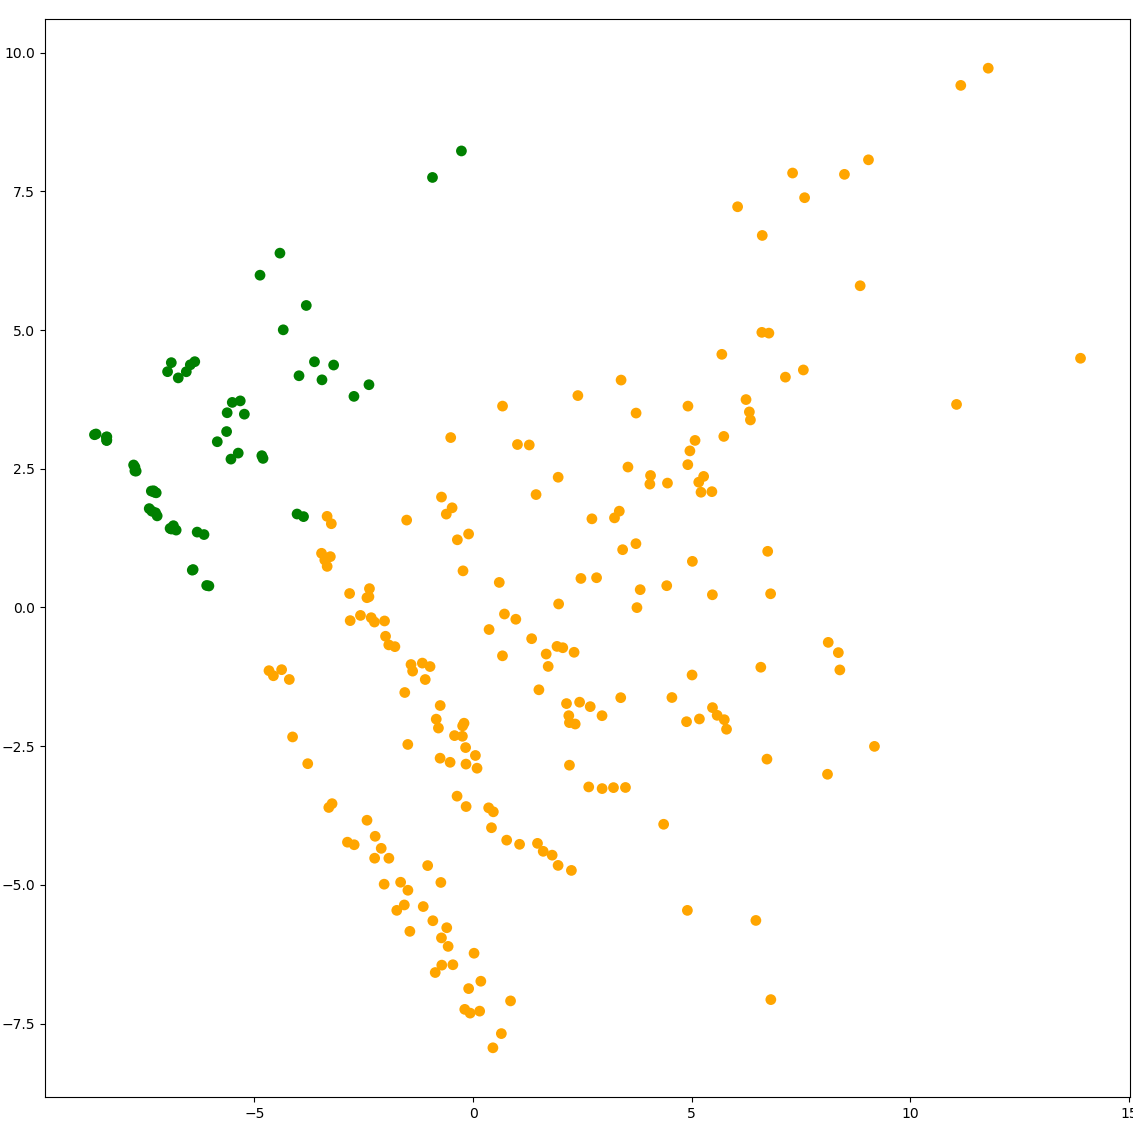
\includegraphics[width=5.5cm, height=5.5cm, keepaspectratio]{./img/cha2_82}
		\caption{Agglomerative clustering}
	\end{subfigure}
	\begin{subfigure}{0.5\textwidth}
		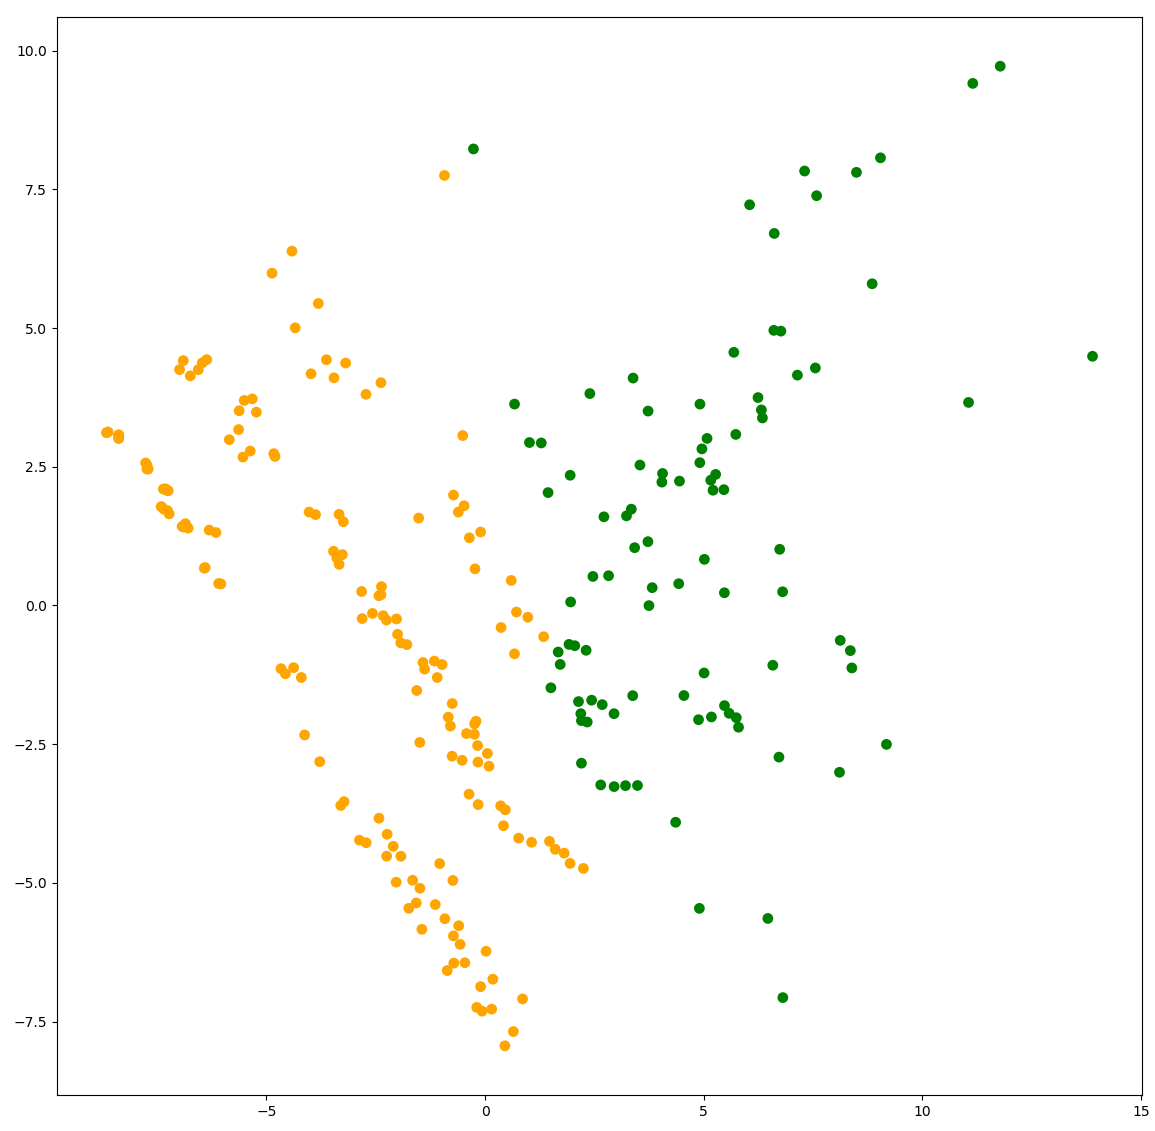
\includegraphics[width=5.5cm, height=5.5cm, keepaspectratio]{./img/km2_82}
		\caption{k-Means}
	\end{subfigure}
\caption{Clustering of the 1882 texts into two classes according to different algorithms.}
\label{fig:cha_km}
\end{figure}

It is important to keep in mind that different algorithms will fit different kinds of data shapes (see Figure~\ref{fig:cha_km}). For instance, agglomerative clustering, since it works by merging the closest clusters one pair at a time will be sensitive to big gaps in the data; thus the clusters will usually have neat borders but possibly strange shapes and inbalanced sizes. On the other hand, k-Means works with geometric shapes (Voronoï diagrams); hence the clusters tend to have more regular shapes but fuzzier borders.

\begin{figure}
\begin{center}
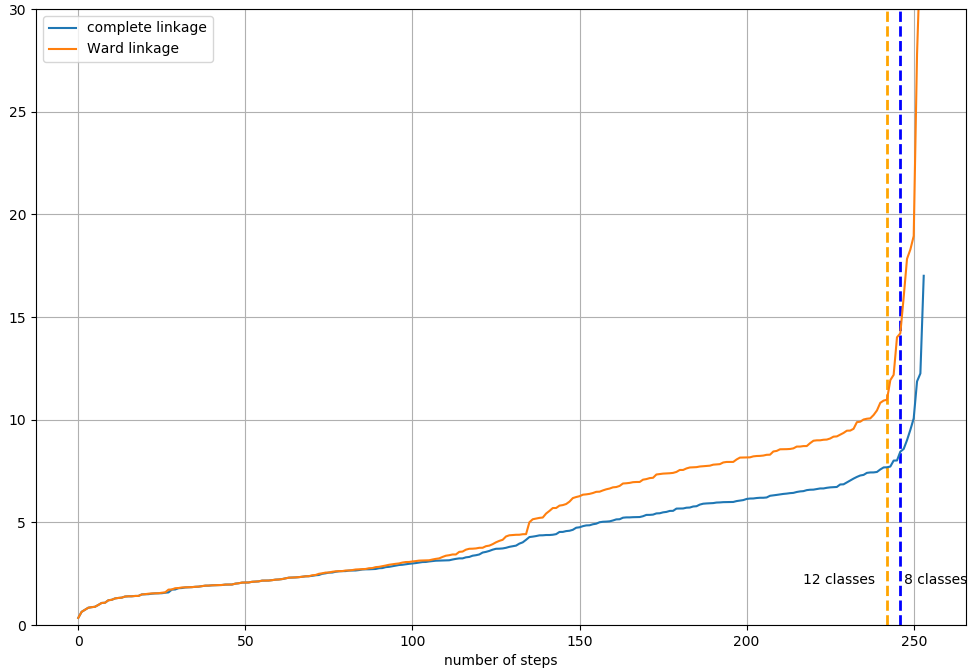
\includegraphics[width=12cm, height=12cm, keepaspectratio]{./img/ward}
\caption{Choice of a number of classes according to some objective function (Ward or complete). Y-axis stands for the value of the objective function; when it rises significantly (the vertical bars stand at the inflection points), it means that further clustering would lead to much less coherent clusters.}
\label{fig:ward}
\end{center}
\end{figure}

When it comes to clustering, the main thing we are looking for is dividing the space into coherent clusters. That means, they should be far apart from each other, which states that the division was necessary ; in addition the distances inside one cluster should remain as small as possible, so that no more subdivision should be required. Thus we can define objective functions that keep that under control. On Figure~\ref{fig:ward} we see (for two different measures) the increase in the function every time we merge two clusters into a single one. In the beginning, increases are pretty moderate, indicating that further clustering is required. At some point there is a sound inflexion, which is the sign that past that limit clusters are too far away from each other to be combined without a big loss of information.

%%%%%%%%%%%%%%%%%%%

\section{Alternative lexicometry tools: coocurrences, topics, embedding}

\subsection*{Simple tools for dealing with changes in vocabulary}

\subsection*{Topic Modeling}

Topic generation model through Latent Dirichlet Allocation (LDA) has been introduced for the first time in 2003 by [REF]. It is based on a bayesian probabilist model, which stems from the following theoretical hypothesis. Before any article is written there exist topics, this word standing for semantic fields, i. e. sets of words that are connected by their meaning. Then the texts are produced by picking words among a small subset of topics with a given probability law. In practice, that means that the texts are the observations who derive from hidden variables, namely the topics, and that statistical correlations in the texts are the direct results of semantic similarities. Thus we expect to find the topics through reverting the generation process. In other words, we want to know the topics as distributions of words and the texts as distributions of topics, conditionally to the observed distribution of words. Unfortunately, computing the universe probability is not tractable so we need to approximate this quantity. Many algorithms have been introduced in litterature to handle this; here we simply use the original one from Blei and al, namely Mean Field variational method (2003).

Let us run a topic model on the whole corpus, with 100 topics. We end up with a lot of topic of great coherence among those, as we can see in Table~\ref{topic_words}.

\begin{figure}
\begin{center}
\begin{tabular}{|ll|ll|}
	\multicolumn{2}{c}{topic 70} & \multicolumn{2}{c}{topic 81} \\
	\hline
	oran & proposition & religieux & élève\\
	rapport & colonisation & établissement & publique\\
	étranger & demande & congrégation & loi\\
	européen & projet & commune & primaire\\
	administration & métropole & état & instruction\\
	commission & tunisien & laïque & enfant\\
	ordre & morinaud & famille & instituteur\\
	constantine & colonie & gauche & enseignement\\
	député & arabe & scolaire & école\\
	\hline
\end{tabular}
\end{center}
\caption{Two topics detected by the algorithm, one about colonization and the second about public instruction}
\label{topic_words}
\end{figure}

Now, the process can been improved in some ways. For instance, there might be several topics that actually deal with the same subjects. Hence we can compute a clustering of topics, in order to merge together those with high proximity, and thus end up with a smaller set of topics, easier to analyze. Since the number of topics is much smaller than the number of words in the vocabulary, the clustering process is easier to visualize as well (See Figure~\ref{fig:dendogram})

\begin{figure}
\begin{center}
\begin{subfigure}{\textwidth}
	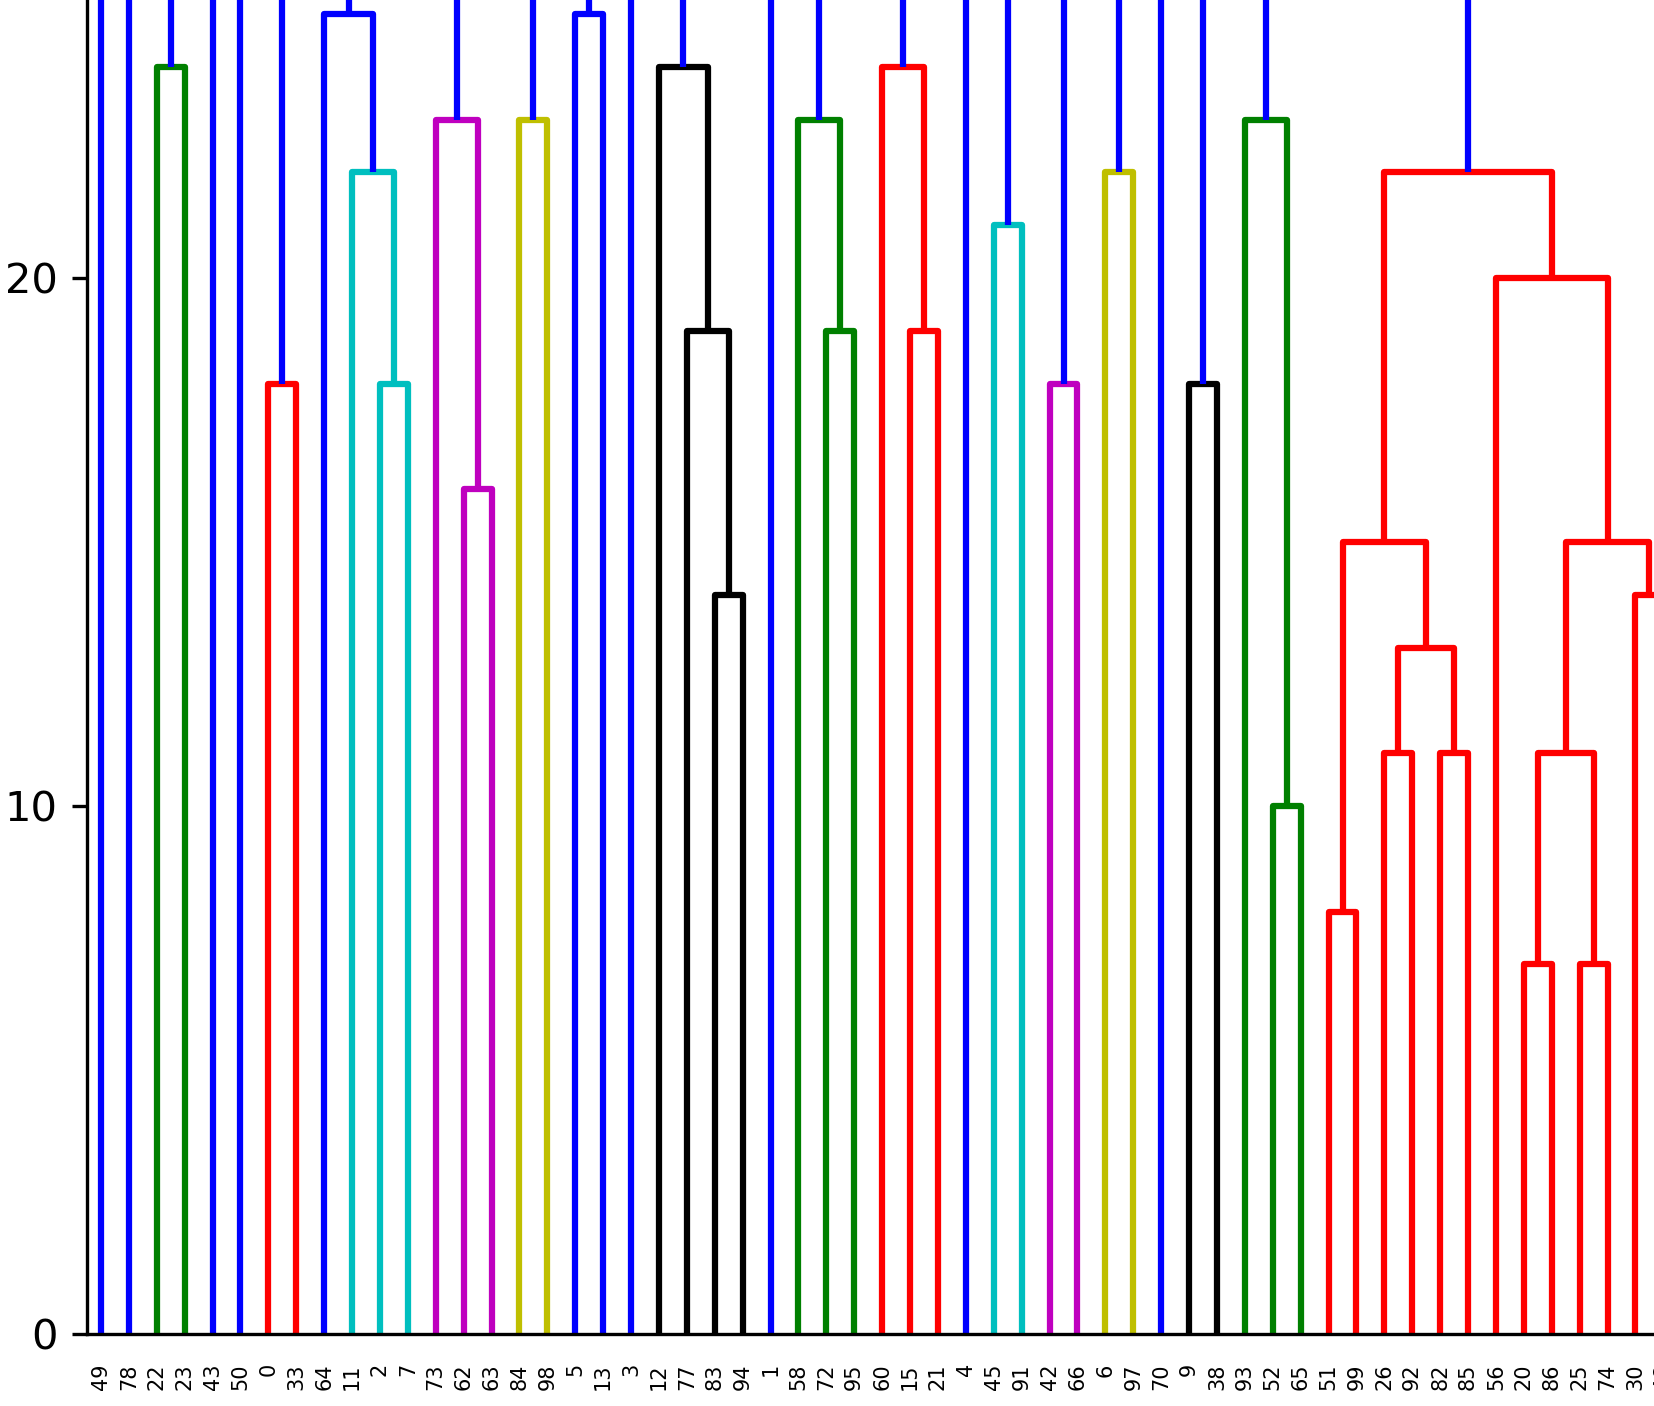
\includegraphics[width=12cm, height=12cm, keepaspectratio]{./img/dendogram}
	\caption{Part of the dendogram of the classification of topics, according to the objective function in the Y-axis (here the distance is equal to the number of different words in two topics). This visualization not only shows when it is necessary to stop the clustering process, as in Figure~\ref{fig:ward}, but also which topics have been merged at every step.}
	\label{fig:dendogram}
\end{subfigure}
\begin{subfigure}{\textwidth}
\begin{center}
\begin{tabular}{|ll|ll|}
	\multicolumn{2}{c}{topic 52} & \multicolumn{2}{c}{topic 65} \\
	\hline
	chambre & internationale & puissance & homme\\
	raison & sécurité & séance & centre\\
	ordre & centre & briand & extrême\\
	problème & monde & demande & angleterre\\
	économique & pacte & monde & conférence\\
	conférence & banc & intérêt & nation\\
	\hline
\end{tabular}
\end{center}
\caption{Details of two topics (in dark green) that are merged at an early stage of the algorithm. They both deal with international relations and have 30 words in common.}
\end{subfigure}
\end{center}
\end{figure}

\subsection*{Assessing the quality of the Model}


%%%%%%%%%%%%%%%%%%%
\section{Evolution with time}

\subsection*{Problem with counting words}



\subsection*{Topics with time}

\subsection*{Dealing with heterogenity}



\end{document}